%% LaTeX Beamer presentation: Climate and Health Prioritization for TASK
\documentclass{beamer}

% Enhanced packages for better styling
\usepackage{graphicx}
\usepackage{hyperref}
\usepackage{booktabs}
\usepackage{bibentry}
\usepackage{multicol}
\usepackage{xcolor}
\usepackage{fontawesome5}
\usepackage{tikz}
\usepackage{tcolorbox}
\usepackage{listings}
\usepackage{enumitem}

% Custom colors
\definecolor{taskblue}{RGB}{0, 83, 155}
\definecolor{tasklightblue}{RGB}{135, 206, 250}
\definecolor{taskgreen}{RGB}{34, 139, 34}
\definecolor{taskred}{RGB}{178, 34, 34}
\definecolor{taskorange}{RGB}{255, 140, 0}

% Theme customization
\usetheme{CambridgeUS}
\usecolortheme{whale}
\setbeamercolor{title}{fg=white, bg=taskblue}
\setbeamercolor{frametitle}{fg=white, bg=taskblue}
\setbeamercolor{structure}{fg=taskblue}
\setbeamercolor{block title}{fg=white, bg=taskblue}
\setbeamercolor{block body}{fg=black, bg=tasklightblue!30}
\setbeamercolor{itemize item}{fg=taskblue}
\setbeamercolor{itemize subitem}{fg=taskorange}

% Title page customization
\title[Climate \& Health for TASK]{\textbf{Decarbonizing Clinical Research:} \\Why Climate and Health Should Be a Strategic Priority for TASK}
\author{\textbf{Craig Parker} \\ \small{Wits Planetary Health, University of the Witwatersrand}}
\date{\textbf{TASK Clinical Trials Afternoon Lecture, 2025}}
\logo{\includegraphics[height=1cm]{example-image}} % Replace with TASK logo

% Custom commands for consistent styling
\newcommand{\highlight}[1]{\textcolor{taskred}{\textbf{#1}}}
\newcommand{\source}[1]{\vspace{0.3cm}\hfill\scriptsize\textcolor{gray}{Source: #1}}

% Custom block environments
\newenvironment{impactblock}{\begin{tcolorbox}[colback=taskorange!20, colframe=taskorange, title=\textbf{Key Impact}]}{\end{tcolorbox}}
\newenvironment{actionblock}{\begin{tcolorbox}[colback=taskgreen!20, colframe=taskgreen, title=\textbf{Action Item}]}{\end{tcolorbox}}

\begin{document}

% Title page with visual enhancement
\begin{frame}[plain]
\titlepage
\begin{tikzpicture}[remember picture, overlay]
\fill[taskblue!30] (current page.south west) rectangle (current page.south east |- current page.south west + (0,1));
\node[anchor=south east, xshift=-0.5cm, yshift=0.3cm] at (current page.south east) {\small\textcolor{white}{Climate \& Health Initiative}};
\end{tikzpicture}
\end{frame}

% Slide 1: Enhanced with icon and impact block
\begin{frame}{Why Climate and Health Matter}
\begin{columns}
\column{0.1\textwidth}
\centering
\faIcon{thermometer-full}\\
\vspace{0.5cm}
\faIcon{globe-africa}\\
\vspace{0.5cm}
\faIcon{hand-holding-medical}
\column{0.9\textwidth}
\begin{itemize}[spacing=0.5em]
    \item Climate change is a \highlight{public health emergency}: rising deaths, heat stress, and malnutrition
    \item LMICs, including South Africa, face disproportionate burdens
    \item Health costs of climate inaction in LMICs: \highlight{US\$8.6--20.8 trillion by 2050}
\end{itemize}
\end{columns}

\begin{impactblock}
Climate change threatens to reverse decades of progress in global health outcomes
\end{impactblock}

\source{The Lancet Countdown, 2023}
\end{frame}

% Slide 2: South Africa's Exposure with visual enhancements
\begin{frame}{South Africa's Exposure}
\begin{columns}
\column{0.65\textwidth}
\begin{itemize}[spacing=0.5em]
    \item \textcolor{taskred}{55\%} increase in heat-related deaths in seniors (1990s--2020s)
    \item \textcolor{taskred}{148 million} labour hours lost in 2022 → \$241 million income loss
    \item Rising vector suitability: malaria \textcolor{taskred}{+94\%}, dengue \textcolor{taskred}{+45\%}
    \item Air pollution from coal → \textcolor{taskred}{10,000+} deaths/year
\end{itemize}
\column{0.35\textwidth}
\begin{tikzpicture}
\pie[radius=1.5]{55/Heat deaths, 28/Labour loss, 17/Air pollution}
\end{tikzpicture}
\end{columns}

\source{Lancet Countdown South Africa Country Profile, 2023}
\end{frame}

% Slide 3: Research Sector's Role with improved layout
\begin{frame}{Research Sector's Role in Emissions}
\begin{columns}
\column{0.6\textwidth}
\begin{itemize}[spacing=0.5em]
    \item Healthcare contributes \highlight{4--5\% of global GHG emissions}
    \item Research activities: \highlight{27.5 Mt CO\textsubscript{2}e/year} from 350,000 trials
    \item Major sources:
\end{itemize}

\begin{center}
\begin{tabular}{lc}
\toprule
\textbf{Source} & \textbf{Contribution} \\
\midrule
Site energy & 38\% \\
Travel & 22\% \\
Lab equipment & 19\% \\
Logistics & 12\% \\
\bottomrule
\end{tabular}
\end{center}
\column{0.4\textwidth}
\includegraphics[width=\textwidth]{example-image-a} % Replace with actual graph
\end{columns}

\source{Nature, 2021: d41586-021-02696-6}
\end{frame}

% Slide 4: Why Funders Care with quote box
\begin{frame}{Why Funders Care}
\begin{tcolorbox}[colback=white, colframe=taskblue, title=\textbf{Wellcome Trust Policy}]
\centering
\textit{"Only fund research conducted in an environmentally sustainable way."}
\end{tcolorbox}

\vspace{0.5cm}
\begin{columns}
\column{0.1\textwidth}
\centering
\faIcon{money-bill-wave}
\column{0.9\textwidth}
\begin{itemize}[spacing=0.5em]
    \item Required to offset travel emissions \& justify design
    \item Sustainability is now part of \highlight{responsible research conduct}
    \item Funding applications require climate impact assessment
\end{itemize}
\end{columns}

\begin{actionblock}
Research proposals without sustainability considerations increasingly face rejection
\end{actionblock}

\source{Wellcome Trust Environmental Sustainability Policy}
\end{frame}

% Slide 5: Strategic Benefits with visual enhancement
\begin{frame}{Strategic Benefits for TASK}
\begin{columns}
\column{0.7\textwidth}
\begin{itemize}[spacing=1em]
    \item \faIcon{chart-line} Strengthens relevance \& resilience of research
    \item \faIcon{handshake} Aligns with global and national climate-health agendas
    \item \faIcon{award} Improves funder competitiveness
    \item \faIcon{dollar-sign} Enhances operational efficiency
\end{itemize}
\column{0.3\textwidth}
\includegraphics[width=\textwidth]{example-image-b} % Replace with WHO logo or relevant image
\end{columns}

\begin{tikzpicture}[remember picture, overlay]
\node[anchor=south east, xshift=-0.5cm, yshift=0.5cm] at (current page.south east) {\includegraphics[width=2cm]{example-image}}; % Replace with relevant logo
\end{tikzpicture}

\source{WHO COP26 Health Programme}
\end{frame}

% Slide 6: What Can TASK Do with improved layout
\begin{frame}{What Can TASK Do?}
\begin{columns}
\column{0.5\textwidth}
\begin{tcolorbox}[colback=taskgreen!10, colframe=taskgreen, title=\textbf{Trial Design \& Operations}]
\begin{itemize}[leftmargin=*]
    \item \textcolor{taskgreen}{▶} Green trial design
    \item \textcolor{taskgreen}{▶} Reduce travel \& shipment
    \item \textcolor{taskgreen}{▶} Cut single-use plastics
\end{itemize}
\end{tcolorbox}

\vspace{0.3cm}
\begin{tcolorbox}[colback=taskblue!10, colframe=taskblue, title=\textbf{Digital Solutions}]
\begin{itemize}[leftmargin=*]
    \item \textcolor{taskblue}{▶} Remote monitoring
    \item \textcolor{taskblue}{▶} Use virtual tools
    \item \textcolor{taskblue}{▶} E-consent \& paperless data
\end{itemize}
\end{tcolorbox}

\column{0.5\textwidth}
\begin{tcolorbox}[colback=taskorange!10, colframe=taskorange, title=\textbf{Lab \& Energy}]
\begin{itemize}[leftmargin=*]
    \item \textcolor{taskorange}{▶} Optimize lab energy use
    \item \textcolor{taskorange}{▶} Audit carbon footprint
    \item \textcolor{taskorange}{▶} Consider renewable energy
\end{itemize}
\end{tcolorbox}

\vspace{0.3cm}
\includegraphics[width=\textwidth]{example-image-c} % Replace with Green Lab logo
\end{columns}

\source{MyGreenLab.org}
\end{frame}

% Slide 7: Lab Sustainability with temperature graphic
\begin{frame}{Lab Sustainability in Action}
\begin{columns}
\column{0.6\textwidth}
\begin{itemize}[spacing=0.8em]
    \item Adjust ULT freezers to \highlight{-70°C} (vs -80°C)
      \begin{itemize}
        \item Saves 30-40\% energy
        \item Sample integrity maintained
      \end{itemize}
    \item Turn off unused equipment during non-working hours
    \item Share large equipment between research groups
    \item Use renewable energy where possible
\end{itemize}
\column{0.4\textwidth}
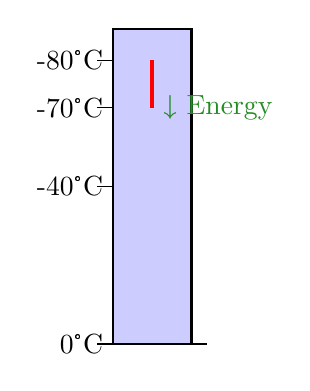
\begin{tikzpicture}
\draw[thick, fill=blue!20] (0,0) -- (0,4) -- (1,4) -- (1,0) -- cycle;
\draw[thick] (-0.2,0) -- (1.2,0);
\foreach \y/\l in {0/0°C, 2/-40°C, 3/-70°C, 3.6/-80°C}
  \draw (-0.2,\y) -- (0,\y) node[left] {\l};
\draw[red, ultra thick] (0.5,3.6) -- (0.5,3) node[right] {\textcolor{taskgreen}{↓ Energy}};
\end{tikzpicture}
\end{columns}

\begin{actionblock}
Simple changes in lab practices can reduce energy use by up to 40\%
\end{actionblock}

\source{Royal Society of Chemistry: Sustainable Laboratories Report}
\end{frame}

% Slide 8: Practical Examples with comparison table
\begin{frame}{Practical Examples}
\begin{tcolorbox}[colback=white, colframe=taskblue, title=\textbf{CRASH Trials Carbon Reduction}]
\begin{tabular}{lccc}
\toprule
\textbf{Metric} & \textbf{CRASH-1} & \textbf{CRASH-2} & \textbf{Reduction} \\
\midrule
Total Emissions & 683 tCO₂e & 187 tCO₂e & 73\% \\
Per-patient & 0.07 tCO₂e & 0.01 tCO₂e & 85\% \\
\bottomrule
\end{tabular}
\end{tcolorbox}

\vspace{0.3cm}
\begin{columns}
\column{0.1\textwidth}
\centering
\faIcon{clipboard-check}
\column{0.9\textwidth}
\begin{itemize}[spacing=0.5em]
    \item Remote monitoring → \highlight{136 tCO\textsubscript{2}e saved}
    \item Lighter packaging, e-data, and batch shipments cut carbon
    \item Decentralized labs reduced sample transport emissions
\end{itemize}
\end{columns}

\source{BMJ Open: Carbon footprint of trials, 2023}
\end{frame}

% Slide 9: Conclusion with call to action
\begin{frame}{Conclusion}
\begin{center}
\Large\textbf{\textcolor{taskblue}{Healing without harming}}
\end{center}

\vspace{0.5cm}
\begin{columns}
\column{0.7\textwidth}
\begin{itemize}[spacing=1em]
    \item Climate-health is \highlight{core} to effective research
    \item Funders expect sustainability \& accountability
    \item TASK can lead on low-carbon trials in Africa
\end{itemize}
\column{0.3\textwidth}

\begin{tikzpicture}
\node[circle, fill=taskgreen!30, minimum size=2.5cm] {\faIcon[regular]{hospital}};
\end{tikzpicture}
\end{columns}

\begin{tcolorbox}[colback=taskblue!10, colframe=taskblue]
\centering
\textbf{Next steps:} Carbon audit → Action plan → Implementation → Leadership
\end{tcolorbox}
\end{frame}

% Slide 10: References with better formatting
\begin{frame}[allowframebreaks]{References}
\begin{thebibliography}{99}
\bibitem{lancet}
\textbf{The Lancet Countdown} (2023).
\textit{The 2023 report of the Lancet Countdown on health and climate change.}
\url{https://www.thelancet.com/countdown-health-climate}

\bibitem{lancetsa}
\textbf{Lancet Countdown} (2023).
\textit{South Africa Country Profile.}
\url{https://www.lancetcountdown.org/south-africa-country-profile}

\bibitem{nature}
\textbf{Wallis, S. et al.} (2021).
\textit{Clinical trials: Rethinking how we reduce carbon emissions.}
Nature, 597(7878), 637.

\bibitem{wellcome}
\textbf{Wellcome Trust} (2023).
\textit{Environmental Sustainability Policy.}
\url{https://wellcome.org/grant-funding/guidance/environmental-sustainability-policy}

\bibitem{who}
\textbf{World Health Organization} (2021).
\textit{COP26 Health Programme.}
\url{https://www.who.int/initiatives/cop26-health-programme}

\bibitem{greenlab}
\textbf{My Green Lab} (2023).
\textit{Laboratory Sustainability Best Practices.}
\url{https://www.mygreenlab.org}

\bibitem{rsc}
\textbf{Royal Society of Chemistry} (2022).
\textit{Sustainable Laboratories Report.}
\url{https://www.rsc.org/sustainable-laboratories-report}

\bibitem{bmj}
\textbf{Roberts I. et al.} (2023).
\textit{Carbon footprint of randomised controlled trials: retrospective study of CRASH trials.}
BMJ Open, 13(5):e070648.
\end{thebibliography}
\end{frame}

% Final slide
\begin{frame}[plain]
\begin{center}
\vspace{1cm}
{\Large\textbf{Thank you}}

\vspace{0.5cm}
{\large Questions?}

\vspace{1cm}
\faEnvelope\ craig.parker@wits.ac.za\\
\faTwitter\ @WitsPlanetaryHealth
\end{center}

\begin{tikzpicture}[remember picture, overlay]
\node[anchor=south, yshift=0.5cm] at (current page.south) {\includegraphics[width=6cm]{example-image}}; % Replace with institution logos
\end{tikzpicture}
\end{frame}

\end{document}